\textbf{Исходный текст:} \\
    Я считаю, что в работе Куртуа-Пепшика есть ошибка. Они переоценили число
    линейно-независимых уравнений. В результате у них нет достаточного количества
    линейных уравнений для решения системы, и [указанный] метод не может взломать
    Rijndael. Он имеет определённые достоинства и заслуживает изучения, но не
    взламывает Rijndael в его нынешнем виде.

\textbf{Ключ:} \\
    3gY5c?>70b>bDNTgFF:FP3<@1S6gYQh3

\textbf{Зашифрованный текст:} \\
    3a48827e37da f48684565bde66660ed14 66fca2f2e 38fa6fbae6bc0403f495 6d83d60f67f11d2 f8aa2856edd 63a163523a298597cd895244f8962a7 74229cdb749aa3cc8a 73d6e73a5ac7de93b698087c04785fc1ad52d e7a1d44d6dc979e63386db42199e724fc2ba1c1f36c cb32e1cf1c95f2ee11f543be9139d2 539d097a32533b75e546f54 9caf980e8c3e2 9bff0ebf6 4f57c62428cb5d46b3cdd4e3765246a704d6d3c9fec65a5cdced3c1 d e208a9c858518ca46fc 1dc88b0864d9b4417e5c650909c686a4f1d4ced 361da722ab53050ffc4a5bb11 416dad0d4ea88d37074c7fc6de88ccca585c3641c f75f9ab9a9d759275f7a51cbb5b3e2f90b28e1fd03a33 d46ad14db9d db87fefaea6f0e9fbc88647af87e12b7e142 58fc8e616fca59e85fd9fa368d7ff87293d37 6d60cd24245e14e67127e272a3e975cb77fe154910284b448c32 8f2ab8558a031cf40a42851d6d7547da8dd437a6c9a8296fbc7a0 5 e4577bb 5a8871c66 c 24efbed405aa529ecf769782bee48 de6c568d4319c30722641add25c87f56c863f 12189f76889a6c5e8b9e7b611881d 056c6f547d969873343afb78172e915825042c3d1a31eea 523de862d49efd647 71bf0f112d0b8199390d675bdab7db1a883822921c71b5d35c4da9a537a24 6e83e1b4ff561163816b570936ae785abfd357be05c2e8ff09afe 1 393e02c1a904a45506a5b797426c84ca46e1f23dbb6d82f2cf674 2c3ccd4 0c56aaa7dfc9f4b63719f2c5998145b498d45561ec5a71ae13cc69bde4258def7 77af971088 abd33b2a6ca8d607342afaa 3afea7b1493f1aad34cae845c21583befd3c2 2d66960c8 5fa1ba7

Результаты работы программы представлены на рисунках~\ref{ris:encode-test-4}-\ref{ris:decode-test-4}.

\vspace{\baselineskip}
\begin{figure}[H]
\center{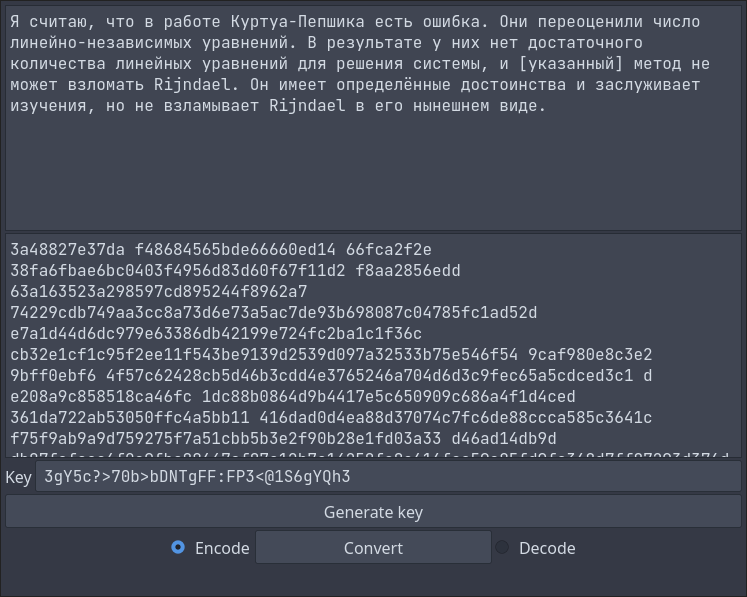
\includegraphics[width=0.8\linewidth]{figures/encode-test-4}}
    \caption{Шифрование}
\label{ris:encode-test-4}
\end{figure}

\vspace{\baselineskip}
\begin{figure}[H]
\center{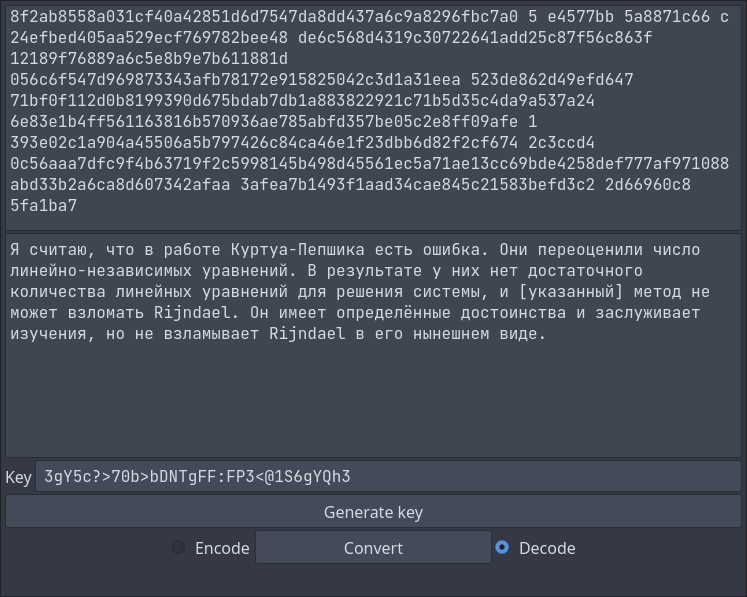
\includegraphics[width=0.8\linewidth]{figures/decode-test-4}}
    \caption{Расшифрование}
\label{ris:decode-test-4}
\end{figure}
